%!TEX root = ../thesis.tex
%*******************************************************************************
%*********************************** First Chapter *****************************
%*******************************************************************************

\chapter{Numerical Methods}  %Title of the First Chapter

\ifpdf
    \graphicspath{{Chapter3/Figs/Raster/}{Chapter3/Figs/PDF/}{Chapter3/Figs/}}
\else
    \graphicspath{{Chapter3/Figs/Vector/}{Chapter3/Figs/}}
\fi

\label{chapter 3}

%**************************************************************************
Building on the theoretical framework established in Chapter 2, we now shift our focus to the numerical methods used to simulate the behavior of plasma in tokamaks. Chapter 3 will detail the specific numerical schemes and techniques employed in our simulations, including the MUSCL-Hancock and MHD-HLLC methods. We will also discuss advanced techniques for divergence cleaning and the handling of rigid body interactions within the plasma. These methods are critical for ensuring the accuracy and stability of our simulations, which are validated through various tests and preliminary results presented in the following chapter.
\section{Numerical Scheme}
\label{section 3.1}
We establish a two-dimensional Cartesian grid and then apply a finite volume method to it. We use a CFL number of $C_{CFL}=0.4$ for two-dimensional space and a dimensional splitting operator $\mathbf{u}_{i,j}^{n+1}={{Y}^{\left( \Delta t/2 \right)}}{{X}^{(\Delta t)}}{{Y}^{\left( \Delta t/2 \right)}}\left( \mathbf{u}_{i,j}^{n} \right)$. The CFL number, $C_{CFL}$, stands for the Courant–Friedrichs–Lewy (CFL) number, which is used to calculate the maximum stable time step for each iteration. For stability, $C_{CFL}$ should be in the range $(0, 1)$ and should not be bigger than 1 in normal cases. This is used to calculate the time steps two-dimensionally computationally through $\Delta t=\frac{C_{CFL} \min(\Delta x, \Delta y)}{a}$, where $a$ is the fastest wave speed. In our case, the fastest wave $a$ is calculated by $a=\max(|v_x|,|v_y|)+c_f$. $c_f$ is the fast magneto-acoustic speed
$$c_f=\sqrt{\frac{1}{2}(c_s^2+c_a^2+(c_s^2+c_a^2)^2-4c_s^2c_a^2cos^2\theta)},$$ where $\theta$ is its propagation direction. $c_a^2 \cos^2 \theta = B_x^2 / \rho$ when updating in the x direction and $c_a^2 \cos^2 \theta = B_y^2 / \rho$ when updating in the y direction. The Alfvén wave speed and the acoustic speed are calculated by $c_a = \frac{|\mathbf{B}|}{\sqrt{\rho}}$ and $c_s = \sqrt{\frac{\gamma p}{\rho}}$. Specifically, when the magnetic field is zero $\mathbf{B}=0$, the fast magneto-acoustic speed equals to the acoustic speed $c_f = c_s$. Here we use a relstive low $C_{CFL}=0.4$ originally to suppress the potential oscillations when waves propagate obliquely. we found that using a higher CFL number, such as 0.8, will also works. The ${X}^{(\Delta t)}$ and ${Y}^{(\Delta t)}$ are the operators that evolve the equation using the conservative update formula (\ref{MHDsystem}) within the time step $\Delta t$ in each direction. They are given by:
\begin{align*}
&{X}^{(\Delta t)}(\mathbf{u}^{n}_{i}) = \mathbf{u}^{n}_{i} - \frac{1}{2} \frac{\Delta t}{\Delta x} \left( \mathbf{f}_{i+1/2}^{n} - \mathbf{f}^{n}_{i-1/2} \right)\ &\text{operator updating in the x direction,}\\
&{Y}^{(\Delta t)}(\mathbf{u}^{n}_{i})= \mathbf{u}^{n}_{i} - \frac{1}{2} \frac{\Delta t}{\Delta y} \left( \mathbf{g}_{i+1/2}^{n} - \mathbf{g}^{n}_{i-1/2} \right)\ &\text{operator updating in the y direction.}
\end{align*}
$\mathbf{f}$ and $\mathbf{g}$ are the fluxes in the x and y directions. The numerical scheme we use to calculate the flux $\mathbf{f}$ or $\mathbf{g}$ is the MUSCL-Hancock method \cite{toro2013riemann} along with the MHD-HLLC solver \cite{li2005hllc}.
\subsection{MUSCL-Hancock}
We use a MUSCL-Hancock method to achieve second-order accuracy in time and space \cite{toro2013riemann}. This method generalizes a first-order finite volume scheme, in our case MHD-HLLC, to second-order accuracy. 
The MUSCL-Hancock method initiates with the MUSCL step, a technique proposed by van Leer \cite{van1979towards}, which is an acronym for Monotonic Upstream-Centered Scheme for Conservation Laws. This method employs linear reconstruction strategies to attain second-order spatial accuracy, effectively leveraging the differences between cell values, denoted as $\Delta_{i+1/2}=\mathbf{u}_{i+1}-\mathbf{u}_i$. Consequently, a slope within cells can be calculated using $\Delta_i=\frac{1}{2}(1+\omega)\Delta_{i-1/2}+\frac{1}{2}(1-\omega)\Delta_{i+1/2}$. Here, $\omega$ serves as a balancing coefficient between minimizing oscillation and enhancing capture, which is crucial for the scheme's upwind bias \cite{li2019weno}. For Euler and MHD cases, a $\omega$ value of 0 is typically chosen to ensure stability. The value of $\mathbf{u}_{i}(x)$ within a cell is determined by $\mathbf{u}_{i}(x)=\mathbf{u}_{i}^n+(x-x_i)\frac{\Delta_i}{\Delta x}$, with $x_i$ representing the cell's center. Slope limiting introduces a limiter to the slope to prevent excessive gradients, defined as ${{\mathbf{\bar{u}}}_{i}}(x)=\mathbf{u}_{i}^{n}+(x-{{x}_{i}})\frac{{\bar{\Delta}}_{i}}{\Delta x}$, where ${{\bar{\Delta }}_{i}}=\xi (r){{\Delta }_{i}}$, and $\xi(r)$ is the applied limiter. The slope limiter used is the Van-Leer limiter \cite{van1979towards}, given by $$\xi(r) = 
\begin{cases} 
0 & r \leq 0 \\
\min\left( \frac{2r}{1+r}, \xi_R(r) \right) & r > 0 
\end{cases}$$, with $r = \frac{\Delta_{i-\frac{1}{2}}}{\Delta_{i+\frac{1}{2}}}=\frac{q_i-q_{i-1}}{q_{i+1}-q_i}, \quad \xi_R(r) = \frac{2}{1+r}
$. Through the MUSCL step, the method facilitates a controlled slope within cells to achieve second-order spatial accuracy. Specifically, it adjusts $$\mathbf{\bar{u}}_i^{R,L}=\mathbf{u}_i\pm \frac{1}{2}\bar{\Delta}_i$$ $$\quad \mathbf{\bar{u}}_{i+1}^{R,L}=\mathbf{u}_{i+1}\pm \frac{1}{2}\bar{\Delta}_{i+1}$$, thereby enabling enhanced accuracy within the numerical scheme.

The Hancock step is utilized to predict the cell interface states at the half-time step, thereby achieving temporal second-order accuracy. In practice, it facilitates in x direction $$\mathbf{\bar{u}}^{L,n+\frac{1}{2}}_{i+1} = \mathbf{\bar{u}}^{L}_{i+1} - \frac{1}{2} \frac{\Delta t}{\Delta x} \left( \mathbf{f}(\mathbf{\bar{u}}^{R}_{i+1}) - \mathbf{f}(\mathbf{\bar{u}}^{L}_{i+1}) \right),$$
$$\mathbf{\bar{u}}^{R,n+\frac{1}{2}}_{i} = \mathbf{\bar{u}}^{R}_{i} - \frac{1}{2} \frac{\Delta t}{\Delta x} \left( \mathbf{f}(\mathbf{\bar{u}}^{R}_{i}) - \mathbf{f}(\mathbf{\bar{u}}^{L}_{i}) \right).$$


\subsection{MHD-HLLC}
The MHD-HLLC solver is originally developed from HLL solver. The HLL approximate Riemann solver was devised by Harten, Lax, and van Leer (HLL) \cite{harten1983upstream}. The HLL method considers an approximation where only two shock waves emerge from a discontinuity, a two-wave model using the two largest signal speeds for bounding. Between these two shocks, there is a homogeneous intermediate state that can be solved using the Rankine-Hugoniot conditions for these two shocks. Such an intermediate state may be too diffusive, neglecting intermediate characteristic fields \cite{toro2019hllc}, such as contact surfaces or shear waves. The assumption of HLL is only appropriate for a hyperbolic system like one-dimensional compressible Euler equations. Toro \textit{et al.} further improved this method by proposing a three-wave model, the HLLC approximate Riemann solver. This considers another intermediate wave, like a contact discontinuity, between these two shocks, separating the intermediate state, with 'C' standing for contact discontinuity \cite{toro1994restoration,toro2013riemann,toro2019hllc}. The HLLC approximate solver greatly enhances the resolution and is extremely popular.

Meanwhile, an MHD extension for HLL, MHD-HLL, was proposed by Janhunen \cite{janhunen2000positive}. This method maintains positivity by allowing small violations of $\nabla\cdot\mathbf{B}=0$. Like HLL, MHD-HLL is too diffusive. Li \cite{li2005hllc} combined the advantages of the MHD-HLL solver and the HLLC approximate Riemann solver and proposed MHD-HLLC. This significantly increases the resolution. However, this method considers a homogeneous magnetic field level and uses an HLL solver for the magnetic field \cite{miki2007large}. The MHD-HLLC approximate solver has not yet considered the characteristic field magnetically, like the rotational discontinuity of the Alfvén waves. Nonetheless, the MHD-HLLC method combines the advantages of the HLLC approximate solver and the MHD-HLL solver. In general, it strikes a good balance between robustness and accuracy. We primarily use the MHD-HLLC approximate solver as our MHD solver fellowing Li \cite{li2005hllc}.

The MHD-HLLC approximate solver posits that a discontinue problem encompasses only three waves: two shock waves and a middle contact discontinuity. In our computational practical, we use this method on finding a solution based on these two states $\mathbf{\bar{u}}^{L,n+\frac{1}{2}}_{i+1}$ and $\mathbf{\bar{u}}^{R,n+\frac{1}{2}}_{i}$, derived from the MUSCL-Hancock step. We take $x$ direction as example. Those fluxes on y are similer. Two estimated shock wave speeds in the $x$ direction, ${{S}_{L}}$ and ${{S}_{R}}$, are calculated in our scheme by $${{S}_{L}}=\min \left(  {{v}_{x,L}} , {{v}_{x,R}}  \right)-\max \left( {{c}_{f,x,L}},{{c}_{f,x,R}} \right),$$ $${{S}_{R}}=\max \left(  {{v}_{x,L}} , {{v}_{x,R}}  \right)+\max \left( {{c}_{f,x,L}},{{c}_{f,x,R}} \right).$$ Here, ${c}_{f,x,L}$ denotes the fast magneto-acoustic speed calculated from the left state. The calculation of fast magneto-acoustic speed is discussed in the beginning of this section \ref{section 3.1}. For the Euler part, Toro \textit{et al.} \cite{toro2013riemann} gave implementation details for HLLC. On the magnetic field, utilizing $\mathbf{B}^{HLLC}=\mathbf{B}^{HLL}$ \cite{li2005hllc} allows for the updating flux calculation: $$\mathbf{f_{i+\frac{1}{2}}}=\mathbf{f^{HLLC} \left( \mathbf{\bar{u}}^{R,n+\frac{1}{2}}_{i},\mathbf{\bar{u}}^{L,n+\frac{1}{2}}_{i+1} \right) }.$$
These generate a computational flux which can be utilized on the updating operator $X^{(\Delta t)}$.
 

\section{Divergence Cleaning Technique}
In section ~\ref{section 2.2}, we discuss several divergence cleaning methods and constrained transport, concluding that a mixture of hyperbolic and parabolic divergence cleaning is accurate enough for our case \cite{vides2013divergence}. We use this divergence cleaning as additional equations evolving alongside the MHD equations. The governing equations are:
\begin{align*}
\frac{\partial \mathbf{B}}{\partial t} +  \nabla \psi = 0 \\
D(\psi) + \nabla \cdot \mathbf{B} = 0
\end{align*}, where a hyperbolic/parabolic operator is 
\begin{equation*}
D(\psi) = \frac{1}{c_h^2} \frac{\partial \psi}{\partial t} + \frac{1}{c_p^2} \psi.
\end{equation*}
The equation for $\psi$ becomes 
\begin{equation*}
\frac{1}{c_h^2} \frac{\partial \psi}{\partial t} + \frac{1}{c_p^2} \psi+ \nabla \cdot \mathbf{B} = 0 .
\end{equation*}
Hence, this forms a hyperbolic system for $\psi$ and $\mathbf{B}$ with a source term
\begin{align*}
\frac{\partial \psi}{\partial t}+c_h^2\nabla \cdot \mathbf{B}&=-\frac{c_h^2}{c_p^2}\psi\\
\frac{\partial \mathbf{B}}{\partial t} +  \nabla \psi &= 0
\end{align*}
The numerical equation for a two-dimensional grid is :
\begin{equation}
    {{\mathbf{U}}_{t}}+\mathbf{f}_x{{(\mathbf{U})}}+\mathbf{g}_y{{(\mathbf{U})}}=\mathbf{S},
\end{equation}
where 
\[
\mathbf{U} = \begin{bmatrix}
\psi \\
B_x \\
B_y
\end{bmatrix}, \quad
\mathbf{f} = \begin{bmatrix}
c_h^2B_x \\
\psi \\
0
\end{bmatrix}, \quad
\mathbf{g} = \begin{bmatrix}
c_h^2B_y \\
0 \\
\psi
\end{bmatrix}, \quad
\mathbf{S}=\begin{bmatrix}
-\frac{c_h^2}{c_p^2} \psi \\
0 \\
0
\end{bmatrix}
.\] We use a Godunov scheme flux to update this equation. Take the flux in x direction as an example:
\begin{equation*}
\mathbf{f}_{i+1/2}=\begin{bmatrix}
0.5c_h(\psi_i-\psi_{i+1})+0.5c_h^2(B_{x,i}+B_{x,i+1}) \\
0.5c_h(B_{x,i}-B_{x,i+1})+0.5(\psi_i+\psi_{i+1})\\
0
\end{bmatrix}.
\end{equation*}

\section{Technique for Rigid Body}
We employ the level set method \cite{andrew2000level} to define the boundaries of rigid bodies. The boundary is specified by setting the zeros of the level set function $\phi$ in the level set method. For the geometries, all we need for iteration are the signed distance, the value of the level set function, and the closest normal vectors. Computationally, we achieve this by giving those closest boundary-pass-by cells an initial $\phi$ and normal vector $\mathbf{n}$ pointing to the closest boundary. Then a fast marching method can be applied to find a plausible $\phi$ and normal vector $\mathbf{n}$ for every cell by iterating through the whole mesh in fictitious time to solve an Eikonal equation $|\nabla\phi|=1$. The normal vector is inherited from the affecting point during the iteration. Hence, the distances and normal vectors are prepared for updating.

After applying the level set method, reflective boundary conditions are then applied to ghost cells that are sufficiently close, specifically where the absolute value of the level set function is less than $GhostCells \times \max(\Delta x, \Delta y)$. The required number of ghost cells, denoted as $GhostCells$, depends on the finite volume scheme utilized. For the MUSCL-Hancock scheme used in our study, we need at least $GhostCells \ge 2$. In our work, the method we used to apply the reflective boundary condition is heavily inspired by Sambasivan \textit{et al.} \cite{sambasivan2009ghost}. We acknowledge and appreciate the significant contributions of their research, which have provided a foundational basis for our implementation.
\subsubsection{Interpolation} For each ghost cell, we need a reflected point as demonstrated in Figure~\ref{fig:Reflective Boundary Condition}. In the figure, the variables at IP1 are needed. The position of IP1, $\mathbf{X}_{IP1}=(x_{IP1},y_{IP1})^T$, can be calculated by the position of P $\mathbf{X}_P=(x_{P},y_{P})^T$, the absolute value of level set function $\left| {{\phi }_{P}} \right|$ and its unit normal vector $\mathbf{N}_P$ \cite{sambasivan2009ghost}:
$$\mathbf{X}_{IP1}=\mathbf{X}_P+2\left| {{\phi }_{P}} \right|\mathbf{N}_P.$$
\begin{figure}
    \centering
    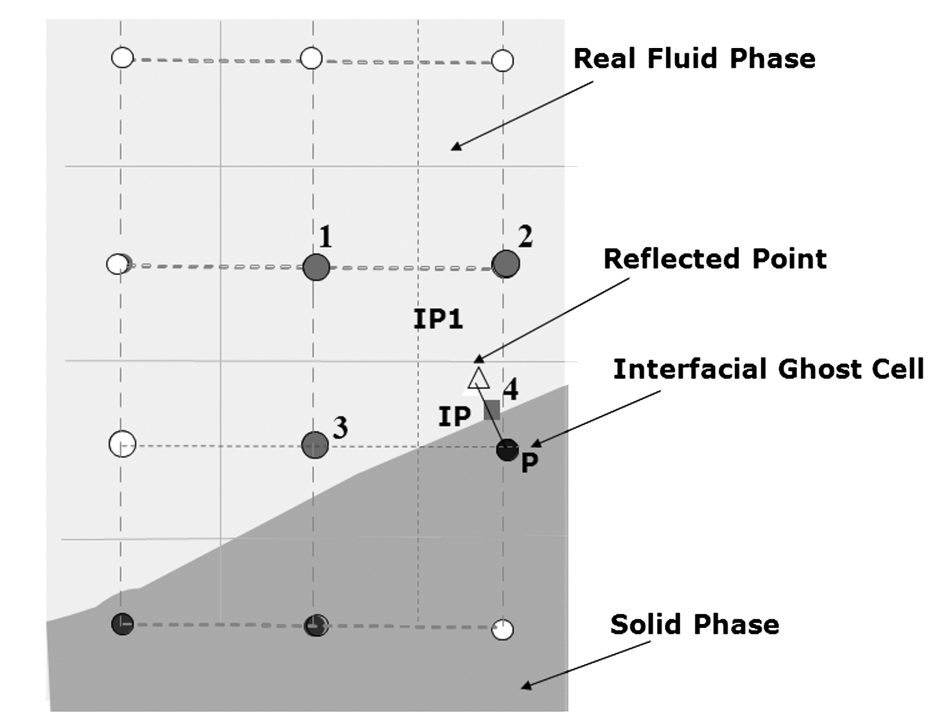
\includegraphics[width=0.5\linewidth]{ReflectiveBC.png}
    \caption[Reflective Boundary Condition]{Reflective Boundary Condition with Bilinear Interpolation Procedure. The reflective boundary condition is applied at point P, requiring variables from the reflected point IP1. Bilinear interpolation necessitates the variables from ghost cell P, where the variables from nearest boundary point IP are instead used. The variables at IP are determined by either Neumann or Dirichlet boundary conditions. This plot is adopted from \cite{sambasivan2009ghost}.}
    \label{fig:Reflective Boundary Condition}
\end{figure}
When interpolating a specific variable $\zeta$ on IP1, the interpolation has the form:
$$\zeta_{IP1}(x_{IP1},y_{IP1})=a_1+a_2x_{IP1}+a_3y_{IP1}+a_4x_{IP1}y_{IP1}.$$
The interpolation points $i=1,2,3,4$ must also satisfy this function with $\zeta_{i}(x_{i},y_{i})=a_1+a_2x_{i}+a_3y_{i}+a_4x_{i}y_{i}.$ Hence, the coefficients $a_{1\sim4}$ can be derived from solving a linear algebra equation:
$$\begin{bmatrix}
    1&x_1&y_1&x_1y_1\\1&x_2&y_2&x_2y_2\\1&x_3&y_3&x_3y_3\\1&x_4&y_4&x_4y_4\\
\end{bmatrix}\begin{bmatrix}
    a_1\\a_2\\a_3\\a_4
\end{bmatrix}=\begin{bmatrix}
    \zeta_{1}\\\zeta_{2}\\\zeta_{3}\\\zeta_{4}
\end{bmatrix}.$$ 
\subsubsection{Handling Invalid Ghost Cells in Interpolation}Some of the necessary points may be the invalid ghost cells. In our case in Figure \ref{fig:Reflective Boundary Condition}, the point 4 is exactly the ghost cell P. In this situation, the closest boundary point IP substitutes. We need to find another equation for IP. Recall the Neumann boundary condition and Dirichlet boundary condition in section \ref{section2.3.1}. When $\zeta$ satisfies the Dirichlet boundary condition of $\zeta_{IP}=\zeta_D$ on boundary $\mathbf{X}_{IP}=(x_{IP},y_{IP})$, we have $$\zeta_{D}=a_1+a_2x_{IP}+a_3y_{IP}+a_4x_{IP}y_{IP}.$$ This gives the linear algebra equation
$$\begin{bmatrix}
    1&x_1&y_1&x_1y_1\\1&x_2&y_2&x_2y_2\\1&x_3&y_3&x_3y_3\\1&x_{IP}&y_{IP}&x_{IP}y_{IP}\\
\end{bmatrix}\begin{bmatrix}
    a_1\\a_2\\a_3\\a_4
\end{bmatrix}=\begin{bmatrix}
    \zeta_{1}\\\zeta_{2}\\\zeta_{3}\\\zeta_{D}
\end{bmatrix}.$$
When $\zeta$ satisfies the Neumann boundary condition of $\partial\zeta_{IP}/\partial\mathbf{n}=\zeta_N$, we have \begin{align*}\frac{\partial\zeta_{IP}}{\partial\mathbf{n}}=\frac{\partial\zeta_{IP}}{\partial x}n_x+\frac{\partial\zeta_{IP}}{\partial y}n_y=\zeta_{N}\\
\zeta_{IP}=a_1+a_2x_{IP}+a_3y_{IP}+a_4x_{IP}y_{IP},
\end{align*}
where $\mathbf{n}=(n_x,n_y)^T$. The partial derivative for $\zeta_{IP}$ gives
$$0+a_2n_x+a_3n_y+a4(n_xy_{IP}+n_yx_{IP})=\zeta_{N}$$ and the linear algebra form 
$$\begin{bmatrix}
    1&x_1&y_1&x_1y_1\\1&x_2&y_2&x_2y_2\\1&x_3&y_3&x_3y_3\\0&n_x&n_y&n_xy_{IP}+n_yx_{IP}\\
\end{bmatrix}\begin{bmatrix}
    a_1\\a_2\\a_3\\a_4
\end{bmatrix}=\begin{bmatrix}
    \zeta_{1}\\\zeta_{2}\\\zeta_{3}\\\zeta_{N}
\end{bmatrix}.$$
\subsubsection{Applying Boundary Condition}
After the interpolation, we can derive the variables on ghost cell P from the reflected point IP1 based on the boundary conditions discussed in section \ref{section2.3.1}. A reflective boundary condition is applied to the velocity field where averages on the boundary are $U_n$ and $U_t$ normally and tangentially:
\begin{align*}
v_{n,P} &= 2U_n - v_{n,IP1} \\
v_{t,P} &= 2U_t - v_{t,IP1}
\end{align*}
For a fixed rigid body, $U_n = 0$. For an ideal plasma with no viscosity, under the slip condition, $U_t = v_{t,IP1}$.

For the magnetic field, if the rigid body is regarded as a perfect conductor, the normal magnetic field and tangential field should satisfy the Dirichlet boundary condition with $B_n = B_{n0}$ and the Neumann boundary condition $\partial B_t / \partial \mathbf{n} = 0$, similar to the 'no-penetration' and 'slip' conditions. Hence,
\begin{align*}
B_{n,P} &= 2B_{n0} - B_{n,IP1} \\
B_{t,P} &= B_{t,IP1}.
\end{align*}
If the rigid body is regarded as an insulator, both the normal component and the tangential component satisfy the Neumann condition:
\begin{align*}
B_{n,P} &= B_{n,IP1} \\
B_{t,P} &= B_{t,IP1}.
\end{align*}
The other scalar variables satisfy the Neumann condition with zero derivatives and are just copies from the reflected point.